\subsection{Mathematischer Hintergrund}

Der Lösungsansatz über die Euler"=Lagrange"=Gleichung ist von der englischen Wikipedia übernommen worden.
\citep{wikidoublependulum}

Die Gleichungen wurden nur um die Konstanten $k_1$ bis $k_5$ erweitert, um sie an unser Pendel anpassen zu können, das keine gleichmäßige Massenverteilung aufweist.

Die Positionen der Pendelarme können durch die zwei generalisierten Koordinaten $\phi_1$ und $\phi_2$ beschrieben werden, die die Winkel der Arme angeben.
Alle Winkel werden relativ zur Ruhelage angegeben, also bedeutet $0^\circ$, dass das Pendel senkrecht nach unten zeigt, während es bei $45^\circ$ nach unten rechts zeigt.
Für die vollständige Angabe des Zustands des Systems ist zusätzlich noch der generalisierte Impuls, hier als $p_1$ und $p_2$ bezeichnet, vonnöten.

Aus den Funktionen $\dot{p}_1$, $\dot{p}_2$, $\phid_1$ und $\phid_2$ setzt sich das System von Differentialgleichungen zusammen, mit dem sich aus dem aktuellen Zustand der Zustand des Systems zu jeder gegebenen Zeit berechnen lässt.
Die Berechnung kann zum Beispiel iterativ mit dem Runge"=Kutta"=Verfahren erfolgen.

\begin{figure}[bht]
  \includegraphics[width=\textwidth]{charts/mathsketch_dia.png}
  \caption{Zeichnung der Pendelarme zur Bedeutung der Längenangaben}
  \label{fig:mathsketch}
\end{figure}

In Abbildung \ref{fig:mathsketch} ist zu erkennen, wie die Längenangaben zu interpretieren sind.
An der ersten Achse ist das Doppelpendel aufgehängt.
$l_{1a}$ ist eine negative Zahl und gibt an, wie lang das erste Pendel auf der Seite ist, an der nicht das zweite Pendel hängt.
$l_1$ gibt den Abstand der beiden Achsen an und $l_{1b}$ beschreibt als positive Zahl die Länge des ersten Pendels in Richtung des zweiten Pendels.
$l_{2a}$ und $l_{2b}$ geben die beiden Längen des zweiten Pendelarms relativ zu seiner Achse an.

Diese Längenangaben sind in den Konstanten $k_1$ bis $k_5$ wiederzufinden, die darauf abzielen, die Eigenschaften des Pendels so genau wie möglich beschreiben zu können, indem zwei Dichtefunktionen $\rho(r)$ über den Abstand $r$ von der jeweiligen Achse für die beiden Pendelarme angegeben werden.

Die Differentialgleichungen lauten wie folgt:
\mathematik
\phid_1 &= \frac{k_4 p_1 - k_5 l_1 p_2 cos(\phi_1 - \phi_2)}{k_1 k_4 + l_1 \cdot (k_3 k_4 - k_5^2 l_1 cos^2(\phi_1 - \phi_2))} \\[0.5\baselineskip]
\phid_2 &= \frac{k_1 p_2 + l1 \cdot (k_3 p_2 - k_5 p_1 cos(\phi_1 - \phi_2))}{k_1 k_4 + l_1 \cdot (k_3 k_4 - k_5^2 l_1 cos^2(\phi_1 - \phi_2))} \\[0.5\baselineskip]
\dot{p}_1 &= -l_1 \phid_1 \phid_2 k_5 sin(\phi_1 - \phi_2) - g k_2 sin \phi_1 - g l_1 k_3 sin \phi_1 \\[0.5\baselineskip]
\dot{p}_2 &= l_1 \phid_1 \phid_2 k_5 sin(\phi_1 - \phi_2) - g k_5 sin \phi_2 \\[0.5\baselineskip]
\mathematikstop

So sind die Konstaten $k_1$ bis $k_5$ definiert:
\mathematik
k_1 &= \int^{l_{1b}}_{l_{1a}} \rho_1(r) \; r^2 \intend r
\qquad && k_2 &= \int^{l_{1b}}_{l_{1a}} \rho_1(r) \; r \intend r \\
k_3 &= \int^{l_{2b}}_{l_{2a}} \rho_2(r) \intend r
&& k_4 &= \int^{l_{2b}}_{l_{2a}} \rho_2(r) \; r^2 \intend r \\
k_5 &= \int^{l_{2b}}_{l_{2a}} \rho_2(r) \; r \intend r \\
\mathematikstop

Hier sind die Formeln für die Berechnung der Energien, die später in der Simulation angezeigt werden, und aus denen auch die Differentialgleichungen hergeleitet wurden. $T$ und $V$ sind die kinetische und die potentielle Energie:
\mathematik
T_1 &= \half k_1 \phid_1^2 & V_1 &= -g k_2 cos \phi_1 \\
T_2 &= \half l_1 k_3 \phid_1^2 + \half k_4 \phid_2^2 + l_1 \phid_1 \phid_2 k_5 cos(\phi_1 - \phi_2) & V_2 &= -g l_1 k_3 cos \phi_1 - g k_5 cos \phi_2 \\
\mathematikstop
\mathematik
T_{Ges} &= T_1 + T_2\\
 V_{Ges} &= V_1 + V_2 \\
E_{Ges} &= T_{Ges} + V_{Ges}\\
\mathematikstop

\subsection{Software}
Wir haben in Haskell eine Simulation geschrieben, die das klassische Runge"=Kutta"=Verfahren anwendet, da Haskell sich gut für Mathematik und den Umgang mit Formeln eignet. Die funktionierende Haskell-Implementierung haben wir dann aus Geschwindigkeitsgründen nach C portiert.
\citep{wikirungekutta}

Die Simulation generiert eine CSV-Datei, in die in regelmäßigen Zeitintervallen die Winkel und die verschiedenen Energien geschrieben werden.
Auf die Winkel wird danach die diskrete Fourier"=Transformation mit einem sich bewegenden Fenster angewendet, um Perioden in der Bewegung erkennen zu können.
Nachdem die Winkel und ihre Transformationen berechnet sind, werden die Daten angezeigt.
In Abbildung \ref{fig:hssim} ist ein Screenshot der Anzeige zu sehen.

\begin{figure}[bht]
  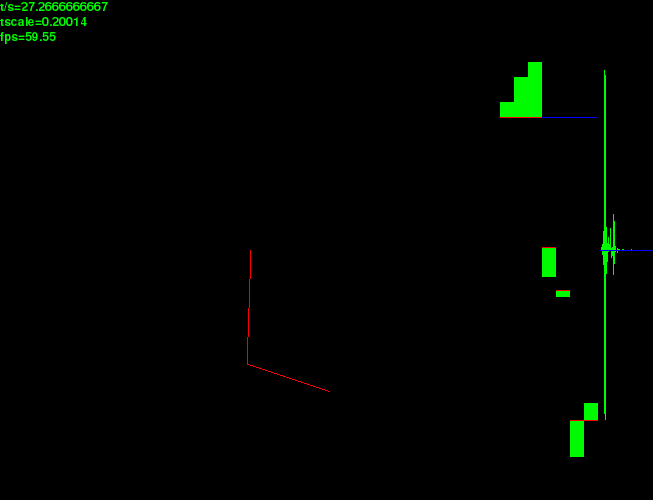
\includegraphics[width=\textwidth]{images/haskell_simulation_fwindow1000_cropped.png}
  \caption{Screenshot der Simulation}
  \label{fig:hssim}
\end{figure}

Zu erkennen ist die aktuelle Position des Pendels als rote Skizze.
Die dicken grünen Balken rechts daneben zeigen auf einer für alle dicken Balken gleichen Skalierung die Energien $T_1$, $T_2$, $T_{Ges}$, $V_1$, $V_2$, $V_{Ges}$ und $E_{Ges}$ in der Reihenfolge von links nach rechts an.
Der blaue Stricht zeigt die Nulllinie an, die roten Striche die Anfangswerte der Energien.
Die potentielle Energie ist anfangs kleiner null, weil der Koordinatenurspung in der ersten Achse liegt und damit die Schwerpunkte der Pendelarme unterhalb des Bezugspunkts liegen.
Die Gesamtenergie $E_{Ges}$ sollte bei einer perfekten Simulation nicht von ihrem Anfangswert abweichen, aber wie zu sehen ist, wächst sie in unserer Simulation stetig.
Dies ist auf die Ungenauigkeiten der numerischen Simulation zurückzuführen.

Rechts neben den dicken Balken ist die diskrete Fourier"=Transformation der Winkel zu sehen.
Oberhalb der blauen Linie wird die Transformation von $\phi_1$ angezeigt, unterhalb die Transformation von $\phi_2$.
Jeder der Balken ist einen Pixel breit und bedeutet eine Frequenz aus dem Ergebnis.
Der Abstand nach rechts vom ersten Balken aus ist proportional zur Frequenz.
Aus dem aktuell zu sehenden Fester ist zum Beispiel für den ersten Pendelarm abzulesen, dass sich das Pendel regelmäßg von rechts nach links bewegt, zu erkennen am rechten Ausschlag, und der zweite Pendelarm eine schwächere aber schnellere Schwingung erzeugt, zu sehen als linker Ausschlag.

Die Transformation des zweiten Pendelarms zeigt eine starke Korrelation mit der Transformation des ersten Pendelarms. Das liegt daran, dass für diese Abbildung eine relativ stark periodische Einstellung des Systems gewählt wurde und der zweite Pendelarm eine dem ersten Pendelarm ähnliche Bewegung durchführt.

